\documentclass{beamer}
\usepackage{amssymb}
\usepackage{amsmath}
\usepackage{stmaryrd}
\usepackage{graphicx}
\usepackage{isabelle}
\usepackage{isabellesym}

%\usepackage{algorithmic}
\usepackage[linesnumbered,ruled,procnumbered,noend]{algorithm2e}
%\usepackage[linesnumbered,ruled,vlined]{algorithm2e}
\usepackage{multicol}
%\usepackage{enumitem}
%\usepackage{program}
 \usepackage{cases}
%\usepackage{ctex}

%%%%%%%%%%%% For Isabelle code
\newlength{\fminilength}
\newsavebox{\fminibox}
\newenvironment{fmini}[1][\linewidth]
  {\setlength{\fminilength}{#1\fboxsep-2\fboxrule}%
   \vspace{2ex}\noindent\begin{lrbox}{\fminibox}\begin{minipage}{\fminilength}%
   \mbox{ }\hfill\vspace{-2.5ex}}%
  {\end{minipage}\end{lrbox}\vspace{1ex}\hspace{0ex}%
   \framebox{\usebox{\fminibox}}}

\newenvironment{specification}
{\noindent\tiny
\tt\begin{fmini}\begin{tabbing}X\=X12345\=XXXX\=XXXX\=XXXX\=XXXX\=XXXX
\=\+\kill} {\end{tabbing}\normalfont\end{fmini}}

\usetheme{Warsaw}
\def \twoSpaces {\ \ }

\def \oneSpace {\ }

\def \oneSpace {\ }
\def \eqc {= }
\def \andc {\wedge }
\def \negc {\neg }
\def \orc {\vee }

\def \dbRight {$\backslash\backslash$}
\def \iInv {iInv}
\def \iR {iR}
\newcommand{\forget}[1]{}

\newcommand\JP[1]{\textcolor{red}{#1}}

\begin{document}

%%-------------------------------------------------


\title{ A Novel Approach to Parameterized Verification of Cache Coherence Protocols}
%\titlerunning{A Novel Approach to Parameterized verification of Cache Coherence Protocols}

\author{Yongjian Li\inst{1} \and  Kaiqiang~ Duan\inst{1} \and Yi~Lv\inst{1} \and Jun Pang\inst{2} \and Shaowei~Cai\inst{1}}

%\authorrunning{Li et al.}

\institute{
State Key Laboratory of Computer Science, China \and
Computer Science and Communications, University of Luxembourg, Luxembourg
}
\frame{\titlepage}
%%-------------------------------------------------

\begin{frame}\frametitle{Problem of Parameterized Verification}
Consdier a protocol $P$, a property $Inv$
\begin{itemize}
\item  $P(N) \models Inv$ for any $N$
\item not just for a single protocol instance  $P(c)\models Inv$
\item Our opinion: parameterized verification is a theorem proving problem
\end{itemize}
\end{frame}

\begin{frame}\frametitle{State of Arts--CMP method}
\begin{itemize}
\item CMP :  parameter abstraction and parameter abstraction
\item Proposed, by McMillan, elaborated by Chou, Mannava, and Park (CMP) , and formalized
by Krstic
\item construction of an abstract instance which can simulate any protocol instance
\item human provides auxiliary invariants (non-interference lemmas)
\end{itemize}
\end{frame}


\begin{frame}\frametitle{State of Arts--Invisible invariants }
\begin{itemize}
\item  Proposed by Amir Pnueli, Sitvanit Ruah, and Lenore Zuck
\item  auxiliary invariants are computed from reachable state set in a finite protocol
instance $P(c)$
\item raw formula translated from BDD
\item  the reachable state set can't be enumerated, e.g., the FLASH protocol
\end{itemize}
\end{frame}



\begin{frame}\frametitle{Two central and difficult problems}
\begin{itemize}
\item  searching auxiliary invariants is not automatic
\item  soundness problem: the theoretical foundation is not mechanized, and there is no  a formal proof
\end{itemize}

\end{frame}

\begin{frame}\frametitle{Our Motivation}

\begin{itemize}
\item automatically searching  auxiliary invariants
\item Formally proving all the things: both the theoretical foundation and case studies
\item A formal proof script as a formal verification product
\end{itemize}
\end{frame}



\begin{frame}\frametitle{An Overview of Our Approach}


\begin{figure}[!t]
\centering
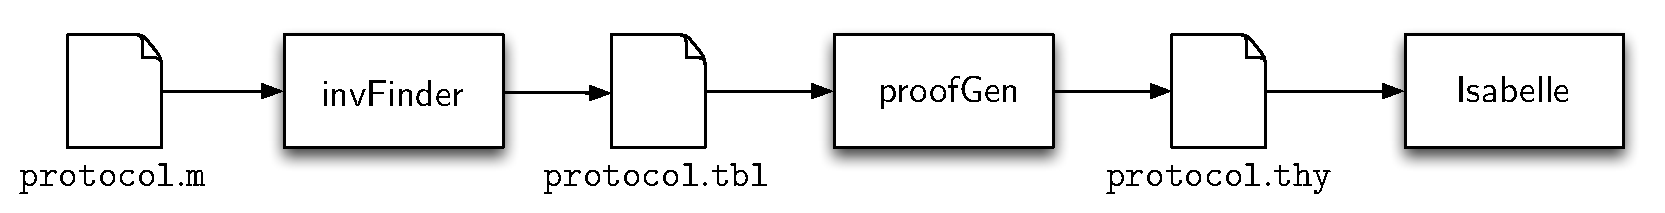
\includegraphics[width=1.0\textwidth]{paraVerifierWorkFlow.pdf}

\caption{The workflow of {\sf paraVerifier}.}
\label{fig:arch}
\end{figure}
\end{frame}



\begin{frame}\frametitle{Some Explanations}

\begin{itemize}
\item {\sf paraVerifier}={\sf invFinder} + {\sf proofGen}

\item protoocl.fl: a small reference instance of the   protocol


\item {\sf invFinder} searches auxiliary invariants automatically

\item   protocol.tbl:  stores the set of ground invariants and a causal relation table

\item {\sf proofGen}: create an Isabelle proof script {\sf protocol.thy} which models and verifies the protocol

\item run Isabelle script to automatically proof-check {\sf protocol.thy}
\end{itemize}

\end{frame}



\begin{frame}\frametitle{Theoretical Foundation-Protocol}
\noindent
A  protocol is formalized as a pair $({\it ini}, {\it rules})$, where
\begin{itemize}
\item ${\it ini}$ is an initialization formula; and
\item  ${\it rules}$ is a set of transition rules. Each rule $r\in {\it rules}$ is defined as
  $g \vartriangleright  S$, where $g$ is a predicate, and $S$ is a
  parallel assignment to distinct  variables $v_i$ with expressions
  $e_i$, where $S$ is  a parallel assignment $S=\{x_i:=e_i | i>0\}$.
\end{itemize}
We write $\mathsf{pre}~r=g$, and $\mathsf{act}~r=S$
  if $r=g \vartriangleright S$.
\end{frame}



\begin{frame}\frametitle{Theoretical Foundation-Causal Relation}



%\begin{definition}
We define the following relations
\begin{enumerate}
\item $\mathsf{invHoldForRule_1}~s ~f ~r \equiv  s \models \mathsf{pre}~ r \longrightarrow s \models \mathsf{preCond}~ f ~(\mathsf{act}~ r)$, where $\mathsf{preCond}~S~f=f[x_i:=e_i]$, which substitutes each
occurrence of $x_i$ by $e_i$;
\item $\mathsf{invHoldForRule_2}~s~ f~ r \equiv  s \models f \longleftrightarrow  s \models\mathsf{preCond}~ f~(\mathsf{act}~ r)$;
\item $\mathsf{invHoldForRule_3}~s~ f~ r ~F \equiv$  $\exists f' \in F$ s.t.
$s \models (f' \wedge (\mathsf{pre}~ r)) \longrightarrow s \models \mathsf{preCond} ~f ~(\mathsf{act}   ~r)$;
\item $\mathsf{invHoldForRule}~s~ f~ r ~F$ represents a disjunction of $\mathsf{invHoldForRule_1}$, $\mathsf{invHoldForRule_2}$
and $\mathsf{invHoldForRule_3}$.
%\item $\mathsf{invHoldForRule}~ f~ r ~F \equiv (\mathsf{invHoldForRule_1} ~f
%  ~r) \lor (\mathsf{invHoldForRule_2} ~f ~r) \lor (\mathsf{invHoldForRule_3}~ f~ r~F)$.
\end{enumerate}
%\end{definition}
\end{frame}

\begin{frame}\frametitle{Theoretical Foundation - Consistency Relation)}


%\begin{definition}
A consistency relation, i.e., $\mathsf{consistent}~ {\it invs} ~{\it ini}~ {\it rules}$,
that holds between a protocol $({\it ini}, {\it rules})$ and
a set of invariants ${\it invs}=\{inv_1,\ldots, inv_n\}$,  is defined as:
%
\begin{itemize}
\item For any invariant ${\it inv} \in {\it invs}$ and state $s$,
if ${\it ini}$ is
evaluated as true at state $s$
(i.e., $\mathsf{formEval}~{\it ini}~s={\it true}$), then ${\it inv}$ is also evaluated as true at the state $s$.

\item For any ${\it inv} \in {\it invs}$,  and $r\in {\it rules}$, and any state $s$,
$\mathsf{invHoldForRule}~{\it inv}~r~{\it invs}$.
\end{itemize}
%\end{definition}


\end{frame}




\begin{frame}\frametitle{Theoretical Foundation - Consistent Lemma}

%\begin{lemma}\label{consistentLemma}%[(Consistency lemma)]
For a protocol $( ini,  rules)$,
we use $\mathsf{reachableSet}~   ini~ rules$
to denote the set of reachable states of the protocol.
Given a set of invariants $ invs$,
we have
$[| \mathsf{consistent}~  invs ~ ini~  rules;
  s \in \mathsf{reachableSet}~  ini~rules|]\Longrightarrow
  \forall  inv \in invs. \mathsf{formEval}~ inv ~s$
%\end{lemma}
\end{frame}



\begin{frame}\frametitle{Key Algorithm of {\sf invFinder}}
\forget{
\begin{algorithm}\label{alg:invFinder}

\caption{Algorithm: $invFinder$}\label{alg:invfinder}

\KwIn{  Initially given invariants $F$, a protocol $\mathcal{P}=<I,R>$ }

\KwOut{A set of tuples which represent causal relations between concrete rules and invariants: }

{
    $A\leftarrow F$;

    $tuples \leftarrow []$;

    $newInvs \leftarrow F$;

    \While{$newInvs$ is not empty}
    {
   $ f \leftarrow newInvs.dequeue$;

   \For {$r \in R$}
   { $paras \leftarrow \mathsf{Policy}(r,f)$;

      \For {$para \in paras$}
     {$cr \leftarrow \mathsf{apply}(r,para)$;

       $newInvOpt,rel \leftarrow \mathsf{coreFinder}(cr,  f, A)$;

        $tuples \leftarrow tuples @[<r, para, f, rel>]$;

       \If{$newInvOpt \neq NONE$}
        {$newInv \leftarrow \mathsf{get}(newInvOpt)$\;
         newInvs.enqueue(newInv)\;
        $A \leftarrow A \cup \{newInv\}$\;
        }

     }
   }
  }
}
\Return $tuples$\;


\end{algorithm}
}
%\begin{algorithm}%\label{alg:invFinder}

\begin{algorithm}[H]

%\caption{Algorithm: $invFinder$}\label{alg:invfinder}


\KwIn {Initially given invariants $F$, a protocol $\mathcal{P}=<I,R>$}
\KwOut {A set of tuples which represent causal relations between concrete rules and invariants:}

$A\leftarrow F$; $tuples \leftarrow []$; $newInvs \leftarrow F$;

\While{$newInvs$ is not empty}
{
   $ f \leftarrow newInvs.dequeue$;

   \For {$r \in R$}
   {
        $paras \leftarrow \mathsf{Policy}(r,f)$;

        \For {$para \in paras$}
        {
            $cr \leftarrow \mathsf{apply}(r,para)$; $newInvOpt,rel \leftarrow \mathsf{coreFinder}(cr,  f, A)$;

            $tuples \leftarrow tuples @[<r, para, f, rel>]$;

            \If{$newInvOpt \neq NONE$}
            {
                $newInv \leftarrow \mathsf{get}(newInvOpt)$\;
                newInvs.enqueue(newInv); $A \leftarrow A \cup \{newInv\}$;
            }
        }
   }

}
\Return $tuples$\;
\end{algorithm}


 \end{frame}



\begin{frame}\frametitle{More on {\sf invFinder}}


\begin{itemize}
\item trying to construct a consistency relation that
guides the tool {\sf invFinder} to find auxiliary invariants

\forget{\item using an oracles that checks whether a ground
formula is an invariant in the small reference model


\item Searching not only auxiliary invariants but also causal relations

\item   protocol.tbl:  storing the searching result}

\item works in a semi-proving and semi-searching way, the result of causal relation can be regarded as key information to construct a concrete proof

\item After fetching an unchecked formula $f$ from $newInvs$, for any rule $r$, $\mathsf{Policy}(r,f)$  generates groups of parameters $paras$  according to $r$ and $f$.

\item     For each parameter $para$ in $paras$,   it is applied to instantiate $r$ into a concrete rule $cr$,  $coreFinder(cr,  f, A)$ is called to check
 whether  a causal relation exists between $cr$ and $f$.
\end{itemize}
 \end{frame}


\begin{frame}\frametitle{Intuition behind $\mathsf{Policy}(r,f)$}


\begin{itemize}
\item Question: How many groups of rule parameters  are needed to instantiate $r$ into concrete rules?

\item The answer will determine how to compute the enough auxiliary invariants and causal relations between these concrete rules and $f$ for generating a proof.

\item For instance, [1], [2], and [3] are three groups which are enough to instantiate $r$ into $\mathsf{crit}(1)$, $\mathsf{crit}(2)$, and $\mathsf{crit}(3)$. But [4] is not needed.

\item Here the generated groups of parameters should cover the typical cases  which are needed in case analysis in a proof of generalized protocol instance.

\item avoiding choosing redundant group of parameters   which are similar  (or equivalent) to each other.
\end{itemize}
 \end{frame}

 \begin{frame}\frametitle{Formalizing $\mathsf{Policy}(r,f)$}

%\begin{definition}
Let $m$ and $n$ be two natural numbers, where $n \le m$,  $L$ and $L'$ are  two  $n$-permutations of $m$,
\begin{enumerate}%[leftmargin=14pt,noitemsep,nolistsep]
\item
$L \sim_m^n L' \equiv (|L| =|L'|=n) \wedge (\forall i. i<|L| \wedge L_{[i]} \le m-n \longrightarrow L_{[i]}=L'_{[i]}) $.

\item $L \simeq_m^n L' \equiv L \sim_m^n L' \wedge   L' \sim_m^n L$.

%\item$[[L]]_{m}^{n} \equiv \{L'. L \in \mathsf{perms}_{m}^{n} \wedge L \sim_m^n L'\}$.

\item $\mathsf{semiP}(m,n,S)\equiv (\forall  L \in \mathsf{perms}_{m}^{n} \exists  L' \in S. L \simeq_m^n L' ) \wedge (\forall  L\in S. \forall L'\in S. L \neq L' \longrightarrow \neg  (L \simeq_m^n L' )$.

\item    A set $S$ is called a quotient of the set $\mathsf{perms}_{m}^{n}$ under the relation $\simeq_m^n$ if    $\mathsf{semiP}(m,n,S)$.
\end{enumerate}
%\end{definition}

Consider a a parameterized rule $r$ with $nR$-parameters, and a concrete invariant formula with $nI$- actual parameters. We only need choose the elements of $\mathsf{semiP}(nR+nI,nR,S)$ to instantiate a rule $r$.

\end{frame}

\begin{frame}\frametitle{Formalizing $\mathsf{Policy}(r,f)$}
\begin{algorithm}[H]
\caption{Computing a quotient of $\mathsf{perms}_{m}^{n}$: $cmpSemiperm$ \label{alg:computeSemiPerms}}%\label{alg:invfinderII}

\KwIn{$m$, $n$     }

\KwOut{A list of permutations $L$}

{
    $L_0\leftarrow \mathsf{perms}_m^n$;$L\leftarrow [] $\;
     \While{$L_0 \neq []$}
      {$para \leftarrow \mathsf{hd}(L_0)$;$L_0 \leftarrow \mathsf{tl}(L_0)$\;
       \If{$\forall para' \in \mathsf{set}(L).  para' \not\simeq_m^n para$}
        { $L\leftarrow L@[para]$\;}
      }
    \Return $L$\;
  %  }
}

%}

\end{algorithm}
$\mathsf{Policy}(r,f)$ is simply calling  $cmpSemiperm((nR+nI,nR)$
\end{frame}

 \begin{frame}\frametitle{Core Searching Algorithm: $coreFinder$}

{\small
\begin{algorithm}[H]

%\caption{Core Searching Algorithm: $coreFinder$}\label{alg:invfinderI}

\KwIn{  $r$, $inv$, $invs$   }

\KwOut{A formula  option $f$, a new causal relation $rel$}

{
    $g\leftarrow $the guard of r, $S\leftarrow $the statement of r,
    $inv'\leftarrow \mathsf{preCond}(inv, S)$\; \label{line:preCondComp}

    \If{$inv=inv'$}
    {
    $relItem\leftarrow (r, inv, invRule_2,-)$\;
    \Return $(\mathsf{NONE},  relItem )$\;
    }
    \ElseIf{$\mathsf{tautChk}(g\rightarrow inv')=true$}
    {
    $relItem\leftarrow (r, inv, invRule_1,-)$\;
    \Return $(NONE,  relItem )$\;
    }
    \Else
    {
    $candidates\leftarrow \mathsf{subsets}(\mathsf{decompose}(\mathsf{dualNeg}(inv')\andc g))$\;
    $newInv\leftarrow choose(chk,candidates)$\;
    $relItem\leftarrow (r, inv, invRule_3,newInv)$\;
    \If{$isNew(newInv,  invs)$}
    {
    $newInv \leftarrow  normalize(newInv)$\;%$ and insert it into the head of $newInvs$\;
    \Return $(\mathsf{SOME}(newInv),   relItem )$\;
    }
    \Else{\Return $(\mathsf{NONE},  relItem )$\;}
    }
}

%}

\end{algorithm}}
 \end{frame}

 \begin{frame}\frametitle{Core Searching Algorithm: $coreFinder$}
After computing the pre-condition $ inv'$ (line \ref{line:preCondComp}) then:
%Algorithm {\sf invFinder-I} performs case analysis on $inv'$:

\begin{itemize}
\item If $ inv=inv'$, meaning that statement $S$ does not change $inv$, then no new invariant is created, and  new causal
relation item marked with tag {\tt invHoldRule$_2$} is recorded
between $r$ and $inv$.% but at this moment there are no new invariants to be added; %for instance, let $ r=\mathsf{crit} (3)$,  $ inv=\mathsf{mutualInv}(1,2)$, thus
%$inv'=\mathsf{preCond}(S,inv)=inv$, then a pair  $ (\mathsf{NONE}, ( crit(3), inv, \mathsf{invHoldRule}_2,\_))$ will be returned, where $NONE$ means no new invariant formula is returned.

\item If $\mathsf{ tautChk}$ verifies that $g \dashrightarrow inv'$ is a tautology, then  no new invariant is created, and
the new causal relation item marked with tag
$ \mathsf{invHoldRule}_1$ is recorded between $r$ and $inv$. %For instance, let $r=\mathsf{crit}(2)$, $inv=\mathsf{invOnXC}(1)$,
% $inv'=\mathsf{preCond}(S,inv)=\neg(\mathsf{false }\eqc \mathsf{true} \andc n[1] \eqc \mathsf{C})$, obviously, $
%g \dashrightarrow inv'$ holds forever because $inv'$ is always evaluated true,
% thus a pair $(\mathsf{NONE},  (\mathsf{crit}(2), inv, \mathsf{invHoldRule}_1,\_))$ will be returned.

\item If neither of the above two cases holds, then a new auxiliary invariant $newInv$ will be constructed, which will make the causal relation $ \mathsf{invHoldRule}_3$  to hold. %The candidate set is $subsets(decompose(dualNeg(inv')\andc g))$, where $decompose(f)$ decompose $f$ into a set of sub-formulas $f_i$  such that each $f_i$ is not of a conjunction form and $f$   is semantically equivalent to $f_1 \andc f_2 \andc ... \andc f_N$. $dualNeg(\negc f)$ returns $f$. $subsets(S)$ denotes the power set of $S$.
\end{itemize}
 \end{frame}


\begin{frame}\frametitle{A fragment of output of {\sf invFinder}}
 \begin{table}[!t]
%\centering \caption{A fragment of output of {\sf invFinder}}\label{label-ground-causal relation} % {\tt
%simpMutual.tbl}
\begin{tabular}{|c|c|c|c|c|  }
\hline
  rule& ruleParas&inv&causal relation &   f'  \\
\hline
  .. & ..&.. &..&.. \\

\hline
  crit  & [1]&mutualInv 1 2& invHoldForRule3 &invOnX$_1$~2 \\
\hline
  crit &[2]& mutualInv 1 2& invHoldForRule3 &invOnX$_1$~1  \\
\hline
  crit & [3]& mutualInv 1 2 & invHoldForRule2  & \\
\hline
  .. & ..&.. &..&.. \\

\hline
  crit  & [1]&invOnX$_1$ 1 & invHoldForRule1 &\_ \\
\hline
  crit &[2]& invOnX$_1$ 1 & invHoldForRule1 &\_  \\
\hline
\end{tabular}
\end{table}
\begin{itemize}
\item invariants and causal relations are in concrete form
\item we need parameterized form (or symbolic form)
\end{itemize}
\end{frame}


\begin{frame}\frametitle{Generalization}
There are two
main kinds of generalization in our work:


\begin{itemize}

 \item generalization of a normalized invariant into a symbolic one.  For instance,  $\negc$(x $\doteq$ true $\andc$ n[1]$\doteq$ C) is generalized into $\negc$(x $\doteq$ true $\andc$ n[$\mathtt{\iInv_1}$]$\doteq$ C).  %This kind of generalization is done with model constraints, which  specifies  that any parameter index should be not greater than the instance size $\mathtt{N}$, and parameters to instantiate a parameterized rule (formula) should be different.

 \item  The generalization of concrete causal relations into parameterized causal relations, which consists of two phases.
  \begin{itemize}
  \item Phase I:  groups of rule parameters  such as [[1],[2],[3]] will be generalized into a list of  symbolic formulas such as $[\mathtt{\iR_1} \eqc \mathtt{\iInv_1},\mathtt{\iR_1} \eqc \mathtt{\iInv_2},  (\mathtt{\iR_1} \ne \mathtt{\iInv_1}) \wedge  (\mathtt{\iR_1} \ne \mathtt{\iInv_2})]$
  \item Phase II: the formula field accompanied with a  relation of kind $\mathsf{invHoldRule_3}$ is also  generalized
 \end{itemize}
\end{itemize}
\end{frame}

\begin{frame}\frametitle{ -From groups of parameters to symbolic formulas}
Let $LR$ and $LI$ be two permutations which represent   rule parameters and invariant parameters, we define:
\begin{itemize}
\item symbolic comparison condition generalized from comparing $LR_{[i]}$ and $LI_{[j]}:$
$ \mathsf{symbCmp}(LR,LI,i,j)\equiv $
 \begin{numcases}{ }
 \mathtt{\iR_i} \eqc \mathtt{\iInv_j} &   if $LR_{[i]}=LI_{[j]}$\ \ \ \ \\
\mathtt{\iR_i} \ne \mathtt{\iInv_j} & otherwise
\end{numcases}
%$symbCmp(LR,LI,i,j)\equiv$ if $equality(LR,LI,i,j)$ then $\mathtt{\iR_i} = \mathtt{\iInv_j}$ else $ (\mathtt{\iR_i} \ne \mathtt{\iInv_j})$

\item symbolic comparison  condition generalized from comparing   $LR_{[i]}$ and with all $LI_{[j]} :$
$\mathsf{symbCaseI}(LR,LI,i)\equiv $\\
\begin{numcases}{ }
   symbCmp(LR,LI,i,j)& if $\exists! j.  LR_{[i]}=LI_{[j]}$\\
   forallForm(|LI|,pf)& otherwise
 \end{numcases}
 where  $pf(j)= \mathsf{symbCmp}(LR,LI,i,j)$, and $\exists!j.P$ is a qualifier denoting there exists an unique $j$ s.t. property $P$;

\item symbolic case  generalized from comparing $LR$ with $LI$ : $\mathsf{symbCase}(LR,LI )\equiv \mathsf{forallForm}(|LR|,pf)$, where $pf(i)= \mathsf{symbCaseI}(LR,LI,i )$;

\item symbolic partition generalized from comparing all $LRS_{[k]}$ with $LI$, where $LRS$ is a list of permutations with the same length: $\mathsf{partition}(LRS,LI) \equiv \mathsf{existsForm}(|LRS|,pf)$,  where $pf(i)= \mathsf{symbCase}(LRS_i,LI)$.

\end{itemize}
\end{frame}

\begin{frame}\frametitle{The result of generalizing lines of Table}
 \begin{table}[htbp]
%\centering \caption{The result of generalizing lines of Table \ref{table:groundCausalRelation} \label{table:symbCausalRelation}} % {\tt
%simpMutual.tbl}
%\vspace{-8pt}
\begin{tabular}{|c|c|c|c|c|  }
\hline
  rule&inv&case & causal relation &   f'  \\
\hline
 % .. & ..&.. &..&.. \\

%\hline
  r& f& $\mathtt{\iR_1} \eqc \mathtt{\iInv_1}$ & invHoldRule3 &invOnXC($\iInv_2$) \\
\hline
  r &f& $\mathtt{\iR_1} \eqc \mathtt{\iInv_2}$ & invHoldRule3 &invOnXC($\iInv_1$)  \\
\hline
   r & f & $\left.
\begin{array}{c}
(\mathtt{\iR_1} \ne \mathtt{\iInv_1})\wedge \\
(\mathtt{\iR_1} \ne \mathtt{\iInv_2})
\end{array}%
\right. $ &invHoldRule2  & \\
\hline
 % .. & ..&.. &..&.. \\

%\hline
%  crit  & [1]&invOnXC(1) & invHoldRule1 &\_ \\
%\hline
 % crit &[2]& invOnXC(1) & invHoldRule1 &\_  \\
%\hline
\end{tabular}
\end{table}
\end{frame}

\begin{frame}\frametitle{\JP{Automatic Generation of Isabelle Proof}}

\begin{itemize}
\item Building formal model and  properties for a protocol  in a theorem prover

\begin{itemize}
\item Building formal model and  properties \JP{\emph{automatically}}

\item Murphi model and computed  invariants $\longrightarrow$  Isabelle model
\end{itemize}

\item Proving that properties hold in the formal model
\begin{itemize}
\item Instead of working interactively,\JP{\emph{ we construct our proof automatically}}

\item lines of symbolic causal table $\longrightarrow$ a proof doing case analysis
\end{itemize}
\end{itemize}
\end{frame}


\begin{frame}\frametitle{A Fragment of Isabelle model}

\begin{itemize}
\item Definition of a formula of an invariant:\\
\emph{
definition inv\_\_1::"nat $\Rightarrow$ nat $\Rightarrow$ formula" where [simp]:\\
"inv\_\_1 p\_\_Inv3 p\_\_Inv4 $\equiv$\\
(neg (andForm (eqn (IVar (Para (Ident ''n'') p\_\_Inv4)) (Const C)) (eqn (IVar (Para (Ident ''n'') p\_\_Inv3)) (Const C))))"\\
}
\item Definition of a lemma: \\
\emph{
lemma critVsinv1:\\
  assumes  a1: $\exists$ \iR1. \iR1 $\le$ N $\wedge$ r=crit \iR1 and \\
  a2: $\exists$  \iInv1 \iInv2. \iInv1 $\le$ N $\wedge$ \iInv2 $\le$ N $\wedge$ \iInv1 $\neq$ \iInv2 $\wedge$ f=inv1  \iInv1 \iInv2\\
  shows  invHoldForRule s f r (invariants   N)\\
}
\end{itemize}
\end{frame}


\begin{frame}\frametitle{A Fragment of Isabelle proof of Lemma critVsinv1}
%\caption{Generating a kind of proof which is according with a relation tag of $invHoldRule_{1-3}$ : rel2proof}\label{lemma:causal relation lemma}
\begin{specification}
1lemma critVsinv1:\\
2  assumes  a1: $\exists$ \iR1. \iR1 $\le$ N $\wedge$ r=crit \iR1 and \\
  a2: $\exists$\iInv1 \iInv2. \iInv1$\le$N $\wedge$ \iInv2 $\le$ N $\wedge$ \iInv1$\neq$\iInv2    $\wedge$ f=inv1  \iInv1 \iInv2\\
3  shows  invHoldRule s f r (invariants
  N)\\
4  proof -\\
   from a1 obtain \iR1 where a1:\iR1 $\le$ N $\wedge$ r=crit \iR1 \\
\twoSpaces   by blast\\
   from a2 obtain \iInv1 \iInv2 where a2: \iInv1 $\le$ N \\
   $\wedge$ \iInv2 $\le$ N $\wedge$ \iInv1 $\neq$ \iInv2 $\wedge$ f=inv1  \iInv1 \iInv2\\
\twoSpaces   by blast \\
5  have iR1=\iInv1 $\vee$ \iR1=\iInv2 $\vee$ (\iR1 $\ne$ \iInv1 $\wedge$  \iR1 $\ne$ \iInv2) \\
  by auto\\

6  moreover\{assume  b1:\iR1=\iInv1\\
7  \twoSpaces have invHoldRule3 s f r (invariants N)\\
 \twoSpaces  \twoSpaces   proof(cut\_tac a1 a2 b1, simp, \\
 rule\_tac x=$\negc$ (x=true $\andc$ n[\iInv2]=C)  in exI,auto)qed\\
8  \twoSpaces then have invHoldRule s f r
(invariants
  N)
by auto\}\\

9  moreover\{assume  b1:iR1=\iInv2\\
10 \twoSpaces have invHoldRule3 s f r (invariants N)\\
 \twoSpaces \twoSpaces   proof(cut\_tac a1 a2 b1, simp, \\
 rule\_tac x=$\negc$ (x=true $\andc$ n[\iInv1]=C  in exI,auto)qed\\
11 \twoSpaces then have invHoldRule s f r (invariants
  N)
by auto\}\\

12   moreover\{assume  b1:(\iR1 $\ne$  \iInv1 $\wedge$   \iR1 $\ne$  \iInv2)\\
13 \twoSpaces have invHoldRule2 s f r  \\
  \twoSpaces \twoSpaces  proof(cut\_tac a1 a2 b1,  auto) qed\\
14 \twoSpaces then have invHoldRule s f r
(invariants
  N)
by auto\} \\

15ultimately show invHoldRule s f r
(invariants N) by blast\\
16qed\\
\end{specification}
\end{frame}

\begin{frame}\frametitle{Experiments}
%\caption{Generating a kind of proof which is according with a relation tag of $invHoldRule_{1-3}$ : rel2proof}\label{lemma:causal relation lemma}
\begin{table}[!t]
\centering
%\caption{\label{Summarization of experiment results}Verification results on benchmarks.}
\vspace{-8pt}
\begin{tabular}{|c|r|r|r|r|}
\hline
Protocols &  \#rules & \#invariants & time (sec.) & Memory (MB) \\
\hline\hline
mutualEx & 4& 5 & 3.25 & 7.3  \\
\hline
MESI & 4& 3 & 2.47 & 11.5  \\
\hline
MOESI &  5& 3 &2.49 & 13.5  \\
%\hline
%Germanish~\cite{cubicle2011}  & 6&3&2.9 & 7.8   \\
%\hline
%German~\cite{Chou2004} & 13 & 24 & 4.09 & 26.7   \\
\hline
German  & 13 & 52 & 38.67 & 14  \\
\hline
FLASH\_nodata & 60 & 152 & 280 & 26  \\
\hline
FLASH\_data & 62 & 162 & 510 & 26  \\
\hline
\end{tabular}
%\vspace{-5mm}
%\vspace{-5pt}
\end{table}

Among them, the former three ones are small, German is medium, FLASH is industrial-scale.
\end{frame}

\begin{frame}\frametitle{Conclusions}

\begin{itemize}
\item   {\sf invFinder}   \emph{generates automatically }  invariants 

\item   {\sf proofGen}     \emph{generates automatically } proofs to prove invariants
 
 \item Our verification output: a formally readable proof. 
 
 \item  Our verification goal:  verifying the protocol in both an automatic and rigorous way
\end{itemize}    
\end{frame}
\end{document}
